\documentclass[12pt]{article}

\usepackage[english]{babel}
\usepackage[utf8]{inputenc}
\usepackage[T1]{fontenc}

\usepackage{geometry}
\geometry{a4paper}

\usepackage{xspace}

\usepackage{graphicx}
\usepackage{enumerate}
\usepackage{verbatim}

\usepackage{float}
\usepackage{wrapfig}
\usepackage{hyperref}
\usepackage{scrextend}
\usepackage{indentfirst}
\linespread{1.2}

\usepackage{color}
\definecolor{darkblue}{rgb}{0,0,0.5}
\definecolor{darkred}{rgb}{0.5,0,0}

\hypersetup{
    colorlinks=true,
    linkcolor=darkblue
}


\graphicspath{{img/}}



\begin{document}
	\newcommand{\tr}{Tracker\xspace}

	{\huge Proposal for assignment 4\\}
	\section{Description}
		The game is a 3D platformer running on a desktop computer.
		The goal of the game is to get to the end of the level.
		The player controls a cube that can move along the platform, jump and shoot.
		The player will have to jump between platforms, shoot down enemies and make sure not to fall into traps.
		\begin{figure}[h!]
			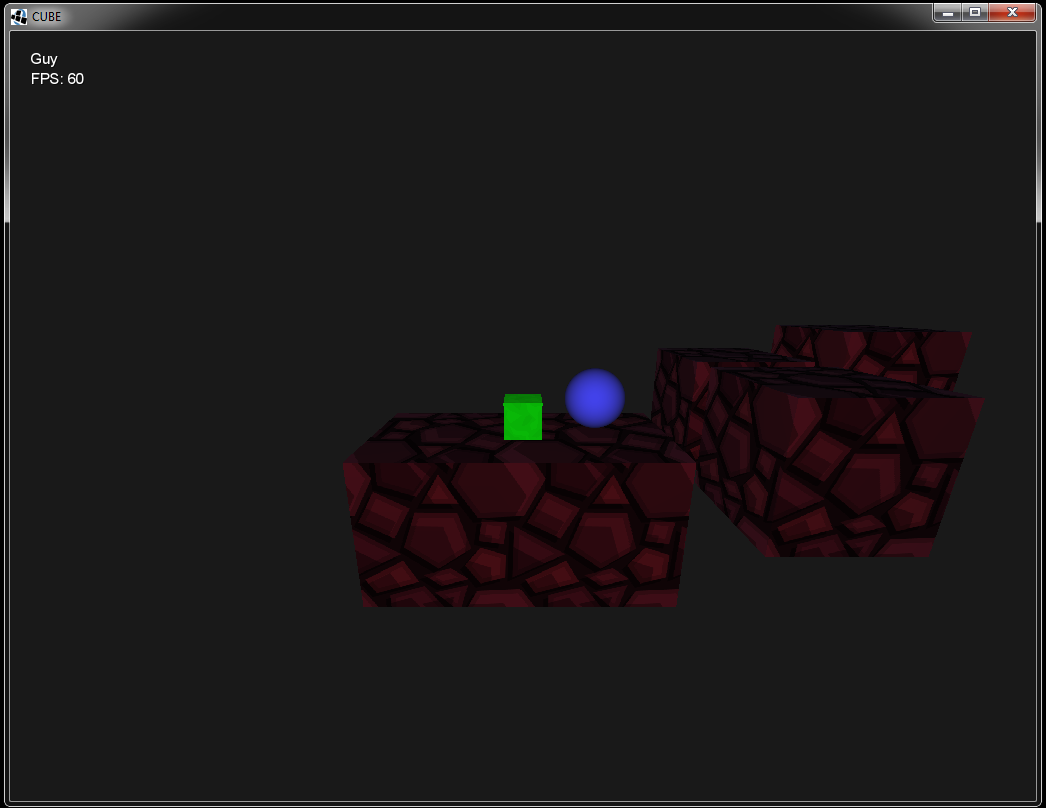
\includegraphics[scale=0.5]{screenshot}
			\caption{Screenshot from prototype}
		\end{figure}

	\section{Design}
		The player will have a camera that is looking at the cube and follows it around, the player moves the cube with the left and right buttons.
		When the cube enters a corner block the camera will rotate 90 degrees as the cube moves over the block. The level should have little light only the
		cube and its surrounding should be well lit, like the player is shining a light at the cube. 
		There will be enemies that will start moving towards the cube when it comes close to them and also enemies that will be on a set course.
		There will be traps such as spike-traps both static and moving.\\


	
	\vspace{5pt}
	\begin{flushright}
	{\large Jóhannes Gunnar Heiðarsson\\}
	JohannesH10@ru.is
	\end{flushright}
	

\end{document}
